\documentclass[10pt,a4paper]{article}

\usepackage[utf8]{inputenc}
\usepackage{cmap}
\usepackage[T1]{fontenc}
\usepackage[scaled=0.95]{helvet}
\renewcommand{\familydefault}{\sfdefault}
\usepackage[portuguese]{babel}
\usepackage[a4paper,margin=1.55cm]{geometry}
\usepackage{graphicx}
\usepackage{xcolor}
\usepackage{enumitem}
\usepackage{needspace}
\usepackage[colorlinks=true,urlcolor=accent,linkcolor=accent,citecolor=accent]{hyperref}

\definecolor{navy}{HTML}{16344A}
\definecolor{accent}{HTML}{16877A}
\definecolor{pale}{HTML}{EDF4F3}
\definecolor{muted}{HTML}{5C6B73}

\setlength{\parindent}{0pt}
\setlength{\parskip}{1pt}
\setlist[itemize]{label={\large\textbullet},leftmargin=1.35em,itemsep=1pt,topsep=2pt}
\urlstyle{same}

\newcommand{\cvsection}[1]{%
    \vspace{11pt}%
    {\large\bfseries\color{navy}#1}\par
    \vspace{2pt}{\color{accent}\rule{\linewidth}{1.2pt}}\par
    \vspace{5pt}%
}

\begin{document}

\noindent
\colorbox{navy}{%
    \begin{minipage}{\dimexpr\textwidth-2\fboxsep\relax}
        \color{white}
        \begin{minipage}[c]{0.72\linewidth}
            {\fontsize{18}{21}\selectfont\bfseries CARLOS ALEJANDRO FREITAS TEIXEIRA}\par
            \vspace{3pt}
            {\large\bfseries\color{pale}Engenheiro de Sistemas | Mestre em Inteligência Artificial}\par
            \vspace{7pt}
            {\small Porto, Portugal \textbar{} E-mail: \href{mailto:carlosfreitasingsistemas@gmail.com}{\textcolor{white}{carlosfreitasingsistemas@gmail.com}} \textbar{} +351 937797609\par}
            \vspace{3pt}
            {\small
                \href{https://github.com/CarlosFreitasING}{\textcolor{white}{GitHub}}
                \textcolor{pale}{\textbar{}}
                \href{https://www.linkedin.com/in/carlos-alejandro-freitas-teixeira-82921a249/}{\textcolor{white}{LinkedIn}}
                \textcolor{pale}{\textbar{}}
                \href{https://carlosfreitas32.wixsite.com/portafolio}{\textcolor{white}{Portefólio}}
            }
        \end{minipage}
        \hfill
        \begin{minipage}[c]{0.22\linewidth}
            \centering
            \fcolorbox{white}{pale}{%
                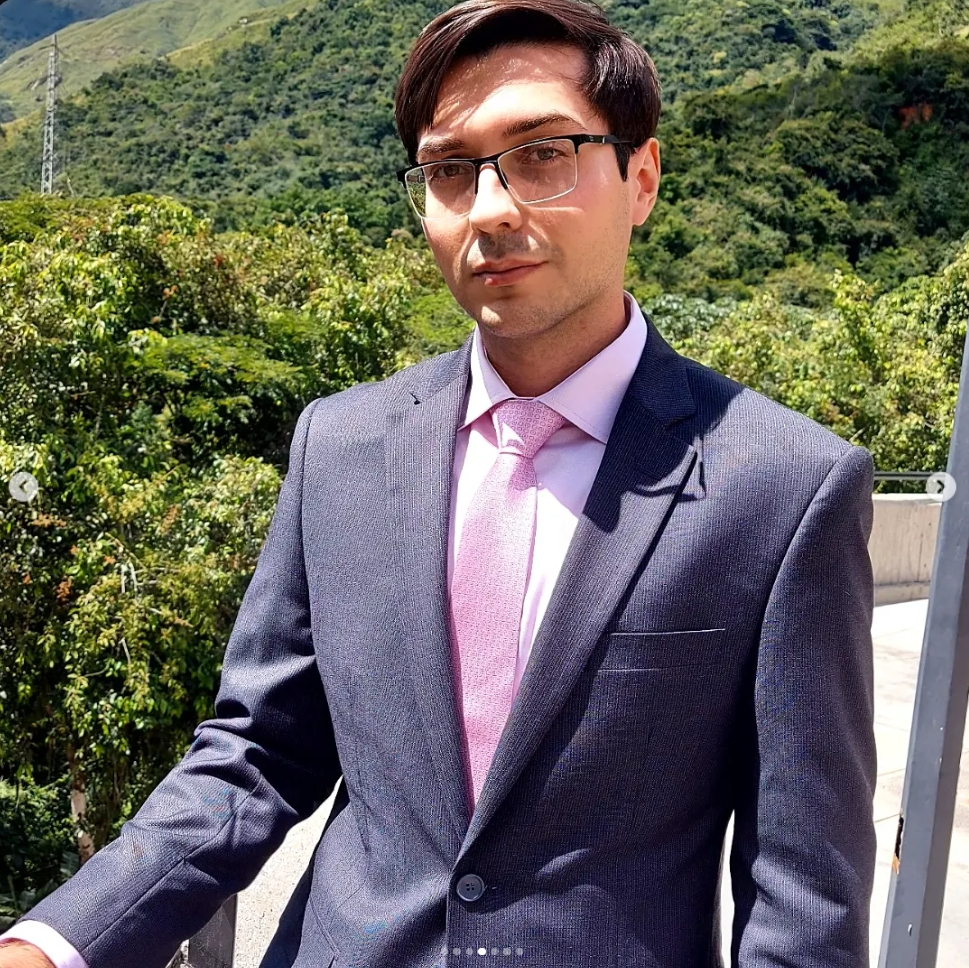
\includegraphics[width=3.2cm,height=3.2cm,keepaspectratio,trim=6cm 12cm 6cm 0cm,clip]{assets/foto.jpeg}%
            }
        \end{minipage}
    \end{minipage}%
}

\cvsection{PERFIL}
\colorbox{pale}{%
    \parbox{\dimexpr\textwidth-2\fboxsep\relax}{%
        Engenheiro de Sistemas e Mestre em Inteligência Artificial, com experiência em investigação aplicada (I\&D) de soluções baseadas em IA. Possuo sólidos conhecimentos em Computer Vision, Machine/Deep Learning, LLMs, Edge AI e Robótica (ROS 2), complementados por experiência prática em desenvolvimento full-stack. Orientado para conceber arquiteturas escaláveis, implementar modelos de inferência local e lançar soluções tecnológicas em contextos reais, orientadas para o utilizador.
    }%
}

\cvsection{EXPERIÊNCIA}

\Needspace{4\baselineskip}
\textbf{\large Investigador e Programador de Inteligência Artificial (I\&D)}\\
{\color{muted}GECAD - ISEP \textbar{} Porto, Portugal}

\vspace{4pt}
\textbf{\color{accent}Projeto CRIARTE \textbar{} out. de 2025 -- presente}\\
Contribuo para um projeto europeu de inovação que procura transformar o setor da construção através de IA, robótica e tecnologias emergentes, no âmbito da Indústria 5.0.
\begin{itemize}
    \item Investigo, treino e avalio modelos de Machine Learning e algoritmos de clustering para analisar dados de sensores vestíveis e identificar padrões associados aos estados fisiológicos dos trabalhadores.
    \item Ajusto modelos YOLO através de fine-tuning para detetar pessoas e estimar a pose humana com sistemas de visão por computador.
    \item Desenvolvo arquiteturas distribuídas baseadas em ROS 2 para integrar sistemas de visão por computador e monitorização fisiológica.
    \item \textbf{Tecnologias:} ROS 2, YOLO, ReID, Computer Vision, Machine Learning, GMM, AHC, Python, C++.
\end{itemize}

\vspace{2pt}
\textbf{\color{accent}Projeto WAI (Wellbeing@Artificial Intelligence) \textbar{} nov. de 2025 -- jun. de 2026}\\
Participei numa iniciativa europeia de investigação que utiliza soluções de Inteligência Artificial para promover o bem-estar dos estudantes e apoiar a gestão da ansiedade e da saúde mental.
\begin{itemize}
    \item Desenvolvi e publiquei a aplicação móvel ``WellBe'' para \href{https://play.google.com/store/apps/details?id=com.caloale.waiv1\&hl=en_US}{Android} e \href{https://apps.apple.com/ie/app/wellbe-journaling-app/id6758772082}{iOS}.
    \item Alcancei uma implementação internacional, com utilizadores em 7 países e mais de 200 transferências.
    \item Implementei modelos de IA com inferência local através de uma arquitetura offline-first para proteger a privacidade dos utilizadores.
    \item \textbf{Tecnologias:} React Native, Expo, EAS Build, SQLite, ONNX Runtime, TinyBERT.
\end{itemize}

\Needspace{4\baselineskip}
\textbf{\large Programador de Software Freelancer}\\
{\color{muted}Remoto \textbar{} out. de 2022 -- presente}
\begin{itemize}
    \item Concebo e desenvolvo soluções full-stack para clientes e empresas, digitalizando e automatizando processos.
    \item Desenvolvo plataformas web e sistemas de gestão, incluindo uma aplicação de fidelização digital para um estabelecimento de restauração (Ver: \href{https://avenidakebab.com/}{Sítio de fidelização}).
    \item Concebo bases de dados, configuro a autenticação de utilizadores e a gestão de permissões e integro serviços através de APIs.
    \item \textbf{Tecnologias:} Angular, React, PWA, iOS/Android, SQL, RLS, APIs e microsserviços.
\end{itemize}

\Needspace{4\baselineskip}
\textbf{\large Programador e Analista Júnior Full-Stack}\\
{\color{muted}INFOCENT C.A. \textbar{} Caracas, Venezuela \textbar{} out. de 2023 -- set. de 2024}
\begin{itemize}
    \item Participei na modernização de uma aplicação legada de processamento salarial para clientes empresariais.
    \item Desenvolvi e implementei novas funcionalidades de frontend e backend para o sistema de processamento salarial.
    \item Efetuei manutenção corretiva, resolvi incidentes e otimizei as funcionalidades do sistema.
    \item \textbf{Tecnologias:} Angular, Spring Boot, Java, SQL, bases de dados relacionais.
\end{itemize}

\Needspace{4\baselineskip}
\textbf{\large Programador de Software e Responsável pela Transformação Digital}\\
{\color{muted}Universidad Metropolitana (UNIMET) \textbar{} Caracas, Venezuela \textbar{} 2021 -- 2022}
\begin{itemize}
    \item Liderei a transformação digital e automatizei o sistema de pedidos académicos, eliminando os estrangulamentos administrativos, otimizando os fluxos de trabalho e suprimindo o processamento manual dos pedidos.
    \item Concebi e desenvolvi uma plataforma web interativa full-stack para autosserviço dos estudantes, com notificações em tempo real e um painel de administração.
    \item Implementei o software em produção e consegui uma adoção sustentada pela comunidade universitária. A plataforma está em utilização desde 2022 (Ver: \href{https://script.google.com/macros/s/AKfycbw3h26r_mjt0jow79RT9dnPaUKZ81dVUsF8qDeEjp7wsRg-ldqHjlB9L0FJYP_Uc_LXUw/exec}{Web Control de Estudio}).
    \item \textbf{Tecnologias:} Google Apps Script, JavaScript, HTML/CSS, Google Sheets, SQL.
\end{itemize}

\cvsection{FORMAÇÃO ACADÉMICA}
\textbf{Mestrado em Inteligência Artificial \textbar{} Instituto Superior de Engenharia do Porto (ISEP)}\\
{\color{muted}Porto, Portugal \textbar{} 2024 -- out. de 2026 (concluído)}\\
Dissertação defendida: ``Análise e Previsão do Estado Fisiológico de Trabalhadores em Obra através de Gémeos Digitais Humanos e Aprendizagem Automática'' (\href{https://drive.google.com/file/d/1xlqiDRtNX2Xj5_9TnHy6inUlAnseSHbF/view?usp=drive\_link}{PDF da dissertação}).

\vspace{5pt}
\textbf{Engenharia de Sistemas \textbar{} Universidad Metropolitana (UNIMET)}\\
{\color{muted}Caracas, Venezuela \textbar{} 2016 -- 2022}\\
Dissertação de licenciatura: ``Aplicação web para a gestão de pedidos e acompanhamento de documentos académicos da Universidad Metropolitana'' (\href{https://unimet.ent.sirsi.net/client/es_ES/default/search/detailnonmodal/ent:\%24002f\%24002fSD\_ILS\%24002f0\%24002fSD\_ILS:132264/one}{registo no catálogo da UNIMET}).

\cvsection{PUBLICAÇÕES E CONFERÊNCIAS}
\begin{itemize}
    \item \textbf{Artigo:} ``A Review of Physiological Monitoring and Prediction in Workers in High-Risk Construction Environments'', apresentado na INISTA 2026 (Guimarães, Portugal, 17--19 de setembro de 2026). Ligações: \href{https://inista2026.di.uminho.pt/pdf/INISTA\_Official\_Program.pdf}{programa oficial} | \href{https://drive.google.com/file/d/1Kh2M0t4dUh3F5vFrKY5sZMfaRxV1H2PT/view?usp=sharing}{PDF do artigo}.
    \item \textbf{Orador convidado:} ``Artificial Intelligence in Health and Mental Health: Challenges, Opportunities and Future Perspectives'', no evento final de divulgação do projeto Erasmus+ WELLBEING@ARTIFICIAL INTELLIGENCE (ISEP, Porto, Portugal, 9--10 de julho de 2026).
\end{itemize}

\cvsection{COMPETÊNCIAS TÉCNICAS}
\begin{itemize}
    \item \textbf{Inteligência Artificial e Dados:} Computer Vision, Pose Estimation (YOLO), ReID, NLP, LLMs, Fine-tuning, Edge AI, ONNX Runtime, PyTorch, OpenCV, Machine Learning (ANN, CNN, RNN), Clustering (GMM/AHC).
    \item \textbf{Linguagens de Programação:} Python, TypeScript, JavaScript, Java, C++, C\#, HTML/CSS.
    \item \textbf{Desenvolvimento e Arquitetura:} React Native, Angular, Spring Boot, ASP.NET, Flutter, arquiteturas Offline-first / Local-first, Serverless, ROS 2, PWA.
    \item \textbf{Bases de Dados e Ferramentas:} PostgreSQL, Supabase, SQLite, MySQL, MongoDB, SQL Server, Firebase, Git.
\end{itemize}

\cvsection{CERTIFICADOS}
Certificado de Inglês de nível C1 e certificado de nível conversacional \textbar{} Fyr Lois \textbar{} 2019 -- 2022.

\vspace{4pt}
Certificados de Competência \textbar{} Universidad Metropolitana \textbar{} 2022
\begin{itemize}
    \item Analista de Sistemas de Informação.
    \item Analista em Conceção e Processamento de Dados.
    \item Assistente de Engenharia em Investigação Operacional (nível básico).
    \item Analista de Redes.
\end{itemize}

\cvsection{IDIOMAS}
\textbf{Espanhol:} nativo \hfill
\textbf{Inglês:} C1 \hfill
\textbf{Português:} conversacional

\end{document}
